\documentclass[a4paper, 11pt]{article} % Font size (can be 10pt, 11pt or 12pt) and paper size (remove a4paper for US letter paper)

\usepackage{cite}
\usepackage{url}
\usepackage{hyperref}

\usepackage[protrusion=true,expansion=true]{microtype} % Better typography
\usepackage{graphicx} % Required for including pictures
\usepackage{wrapfig} % Allows in-line images

\usepackage{mathpazo} % Use the Palatino font
\usepackage[T1]{fontenc} % Required for accented characters
\linespread{1.05} % Change line spacing here, Palatino benefits from a slight increase by default

\makeatletter
\renewcommand\@biblabel[1]{\textbf{#1.}} % Change the square brackets for each bibliography item from '[1]' to '1.'
\renewcommand{\@listI}{\itemsep=0pt} % Reduce the space between items in the itemize and enumerate environments and the bibliography

\renewcommand{\maketitle}{ % Customize the title - do not edit title and author name here, see the TITLE block below
\begin{flushright} % Right align
{\LARGE\@title} % Increase the font size of the title

\vspace{50pt} % Some vertical space between the title and author name

{\large\@author} % Author name
\\\@date % Date

\vspace{40pt} % Some vertical space between the author block and abstract
\end{flushright}
}

%----------------------------------------------------------------------------------------
%	TITLE
%----------------------------------------------------------------------------------------

\title{\textbf{Quadcopters and Drones}\\ % Title
The Start of Making One Yourself} % Subtitle

\author{\textsc{Anders Dahl}} % Author

\date{\today} % Date

%----------------------------------------------------------------------------------------

\begin{document}

\maketitle % Print the title section

\vspace{30pt} % Some vertical space between the abstract and first section

%----------------------------------------------------------------------------------------
%	ESSAY BODY
%----------------------------------------------------------------------------------------

\section*{Introduction}

Radio controlled quadcopters are becoming ever more popular. This paper will address some important aspects of building one yourself. What features should be implemented in hardware and software? What programming languages are useful for quadcopters? How does this technology bring on new safety and ethical issues?

%------------------------------------------------

\section*{The Quadcopter}

\subsection{Hardware Implementation}

Field-programmable gate arrays (FPGAs) are great for time-critical concurrent processing functions; thus, hardware programming could be used for flight control and image processing. If the drone was produced on a mass scale, optimizing flight control using the hardware could save a great deal of money. As far as image processing, the FPGA could compress, crop, and scale the camera's output before sending it to the monitor feed. These repetitive tasks could utilize optimized hardware to ultimately cut down on costs.

\subsection{Software Implementation}

Developers need the ability to add custom scripts and navigational features to the drone. For example, a script could assign a button to perform a flip or side-way maneuver. Or, it could express a navigational path for the drone to take. Overall, a developer should have full control over the drone and be able to shutoff the optimizations in hardware if necessary. The software side should allow the programmer to customize the drone as he sees fit. \cite{DIY} 

\subsection{The FPGA Board}

The Terasic Technologies P0082 Cyclone IV is a reliable, tested board with a mature set of technologies backing it up. Allowing for features to be completed in either hardware or software, it is a flexible board giving a wide range of implementation options. Not to mention, it comes with plenty of processing power. \cite{Board} The board and open source libraries will be the brain behind the quadcopter. \cite{DIY} 

\subsection{Software Programming - C/C++, Python}

The processor would most likely utilize C/C++. Using low-level languages, the developer would get close to the hardware. That being said; however, if there are open source programs or a better tool for the job then those would most likely be used. No option is off the table. GitHub has all types of open-source modules related to drones. A scripting language such as python could deem to be the best fit for some parts.

\subsection{Hardware Programming - VHDL}

At the root, VHDL would be used to program the hardware. It is a commonly used hardware description language (HDL), and many other HDLs generate VHDL code. For example, Python's MyHDL could be used for such a purpose. It allows the developer to use an environment that they are comfortable with while developing VHDL code. VHDL is a mature technology that will provide a good set of options for programming hardware. It will be used to adapt the hardware to the drone's needs accordingly.

\subsection{Safety Issues}

\begin{wrapfigure}{h}{0.4\textwidth} % Inline image example
\begin{center}
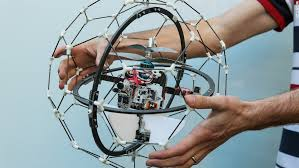
\includegraphics[width=0.40\textwidth]{cage.jpeg}
\caption{Cage Around Drone \cite{Drone}}
\end{center}
\end{wrapfigure}

Quadcopters should not be handled like toys. It is important to adhere to the proper safety rules - major issues can occur otherwise. Designers should think about adding a cage or other protective gear to the drone. All parts should be properly secured and protected from the environment. A caged net surrounding the quadcopter limits the damage if a crash does occur; however, in the end, it is up to the person controlling the drone to take the proper safety precautions. \cite{Safety}

\begin{description}
\item [Care for the Technology] Always make sure the quadcopter is properly secured. There should be no loose parts. Do not fiddle with the rotors when drone is on. \cite{Safety}
\item [Fly Safely] Do not fly near people, houses, or objects. You do not want to injure someone or cause property damage. \cite{Safety}
\item [Keep Direct Line of Sight] A person not in total control of their quadcopter could be reckless. Even if a camera is used, the drone should always be visible to the person controlling it. \cite{Safety}
\item [Always Stay below 400 ft.] 
Airplanes are required by law to fly above 500 ft. You would not want to find yourself in a situation where your drone hit an airplane. It goes without saying, do not fly near an airport. \cite{Safety}
\end{description}

\subsection{Ethical Issues}

Drones come with their own set of ethical issues.

\begin{description}

\item [Privacy] Drones could be used to infringe on a person's privacy. Able to reach a variety of different areas, a quadcopter could be used to look into windows. The user of the drone should never intrude. \cite{Safety}

\item [Safety] Drones can be a danger to people and property if used hazardously. This begs the question of whether they should be allowed in certain areas or near events. \cite{Safety}

\item [Noise] Some quadcopters can be noisy. Should they be banned from areas that try to maintain a peaceful atmosphere such as at a national park? \cite{Safety}

\end{description}

%------------------------------------------------

\section*{Conclusion}

Drones will only become more popular. It is important to integrate them into our society safely and ethically. Hardware and software both play an important role in drone construction. Hardware optimizations often lead to cheaper build costs if the drone is mass produced. It is important to see the benefits and consequences of implementing a feature in hardware or software. Often, there are many ways to solve a problem, but one way may be more beneficial for that specific task. The same goes for choosing what programming language to use.

%----------------------------------------------------------------------------------------
%	BIBLIOGRAPHY
%----------------------------------------------------------------------------------------

\bibliographystyle{ieeetr}
\bibliography{research_paper}{}

%----------------------------------------------------------------------------------------

\end{document}